% ****************************************************************************************************
\chapter{Causal Loop Diagram -- A qualitative Model}\label{ch:cld}
% ****************************************************************************************************

\begin{flushright}{\slshape    
	We shape our buildings; thereafter, our buildings shape us.} \\ \medskip
	--- Winston Churchill
\end{flushright}

Within this chapter, the crucial interdependencies -- high-leverage interventions and policies -- between the above described classification criteria respectively characteristics are reveled and illustrated using the concepts of system dynamics, more specifically by means of a \ac{CLD} and thereby also answering the \thref{srq2}. System dynamics is an approach to study complexity and was originally developed at the \ac{MIT} by Jay W. \citet{Forrester1961}. John D. \citeauthor{Sterman2000} applied system dynamics to business and organizational problems -- a comprehensive \citep{Sterman2000} as well as brief \citep{Sterman2001} introductory guides are provided. Within this thesis the notation and guidelines provided by John D. \citeauthor{Sterman2000} are used (please refer to the above mentioned sources). The ulterior motive behind \ac{CLD} is the simplification of reality by defining suitable model boundaries. \acp{CLD} \textit{"can never be comprehensive (and you shouldn't try: modeling is the art of simplification). They are also never final, but always provisional"} \citep[p. 166]{Sterman2000}. An important aspect of causal relationships within \acp{CLD} which should always bear in mind, is that the causal relations are modeled ceteris paribus (literally translated as "with other things the same" or "all other things being equal or held constant") \footnote{\textit{"A positive link means that if the cause increases, the effect increases above what it would otherwise have been, and if the cause decreases, the effect decreases below what it would otherwise have been. [\ldots] A negative link means that if the cause increases, the effect decreases below what it would otherwise have been, and if the cause decreases, the effect increases above what it would otherwise have been"} \citep[p. 139]{Sterman2000}.}.

In the beginning of this chapter, the causal relationships for the generic customer segment in the \ac{PaaS} domain are discussed in Section \ref{ch:cld:cs}. Thereafter, interdependencies between the five identified customer segments are presented in Section \ref{ch:cld:csi}. At the end of this chapter, the overall \ac{CLD} is depicted and explained in Section \ref{ch:cld:bp}.

\section{Generic Customer Segment}\label{ch:cld:cs}

\section{Customer Segment Interdependencies}\label{ch:cld:csi}

\section{The Big Picture}\label{ch:cld:bp}


\begin{figure}[htb]
	\centering
	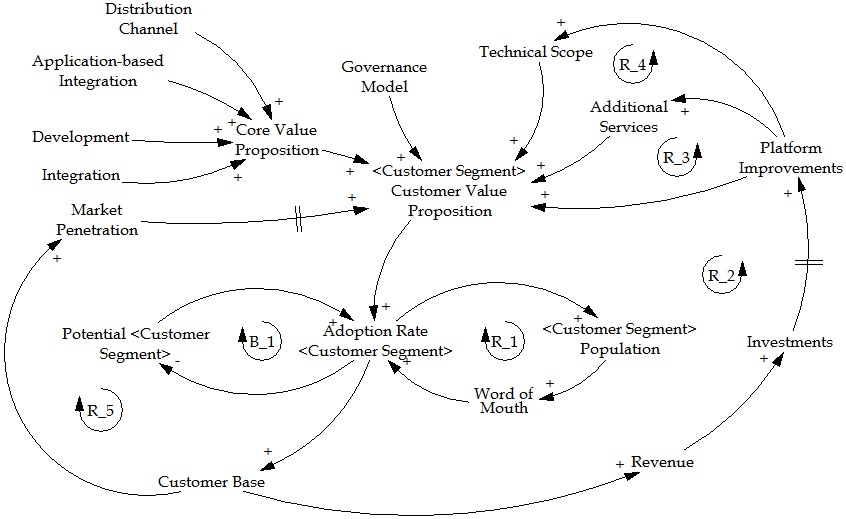
\includegraphics[width=\textwidth]{gfx/cld_customerSegment}
	\caption{Causal Loop Diagram -- Customer Segment}
	\label{fig:cld_cs}
\end{figure}




\begin{itemize}
	\item kein market share der Konkurrenz, da zu umfassend, wird erstmal vernachl�ssig; �ber die initialen potential customers (initial value) kann dies rudiment�r abgebildet werden (new entrants, markts�ttigung, market share competition, marketanteil
	\item CVP f�r jede Kundengruppe
	\item keine Kosten, da zu komplex (hosting Standort, Anzahl Developer)
	\item GOV, TS,.... mit unterscheidlichen gewichten zu CVP
	\item CoVP hat unterschiedliche Auswirkungen auf die Kunden CVP
\end{itemize}


